%\documentclass{article}
%\usepackage{wasysym}
%\usepackage{graphicx}
%\usepackage{bm}
%\usepackage{psfig}
%\newcommand{\bc}{\begin{center}}
%\newcommand{\ec}{\end{center}}
%\newcommand{\be}{\begin{equation}}
%\newcommand{\ee}{\end{equation}}
%\newcommand{\bea}[1]{\begin{eqnarray}\label{#1}}
%\newcommand{\eea}{\end{eqnarray}}
%\newcommand{\bua}{\begin{eqnarray*}}
%\newcommand{\eua}{\end{eqnarray*}}
%\newcommand{\infint}{\int_{-\infty}^{\infty}}
%\newcommand{\dd}[2]{{{d#1}\over{d#2}}}
%\newcommand{\ddt}[1]{\dd{#1}{t}}
%\newcommand{\dddt}[1]{\dd{^2#1}{t^2}}
%\newcommand{\aver}[1]{\langle{#1}\rangle}
%\def\cl#1{{\cal #1}}               % for caligrafic letters
%\def\labs{\mid\!}
%\def\rabs{\!\mid}
%\begin{document}
\section{Lecture notes 5: Diffraction}

Let us now consider how light reacts to being confined to a given aperture. The resolution 
of an aperture is restricted due to the wave nature of light: as light passes through any 
opening it is {\it diffracted} and the wave fronts spread out in a shape given by the 
envelope of Huygens's secondary wavelets which radiate spherically outwards from all points on 
a wave front. These waves travel along every path, from the source to the point of observation,
where they are added together only giving a significant net contribution when they add 
coherently in phase. 

\noindent (In the following I will follow Kip Thorne's lecture notes found at 
\newline{\tt www.pma.caltech.edu/Courses/ph136/yr2004}.)

\subsection*{Helmholtz-Kirchhoff Integral}

Let us restrict attention to the simplest (and, luckily the most
useful) case: a monochromatic scalar wave 
\[
\psi=\psi({\mathbf x})e^{-i\omega t}
\]
with field variable $\psi$ of frequency $\omega=ck$ which satisfies Helmholtz's equation
\be
\nabla^2\psi+k^2\psi=0
\label{eq:helmholtz}
\ee
except at the boundaries. $\psi$ is generally a real physical value, but for convenience we will
use a complex representation. The wave is monochromatic and non-dispersive and the medium is
isotropic and homogeneous so that $k$ can be treated as a constant\footnote{Each of these 
assumptions can be lifted at the cost of introducing technical complications.}. This formalism
is valid for weak sound waves in a fluid and is fairly accurate for the propagation of 
electromagnetic waves in vacuum or in a medium with a constant dielectric constant $\epsilon$. 
In the latter case $\psi$ can be considered as one of the Cartesian components of the electric
or magnetic field vector, e.g. $E_x$ or $B_y$. In vacuum Maxwell's equations imply that 
$\psi=E_x$ satisfies equation~\ref{eq:helmholtz}. 

\begin{figure}[th!]
%  \hfil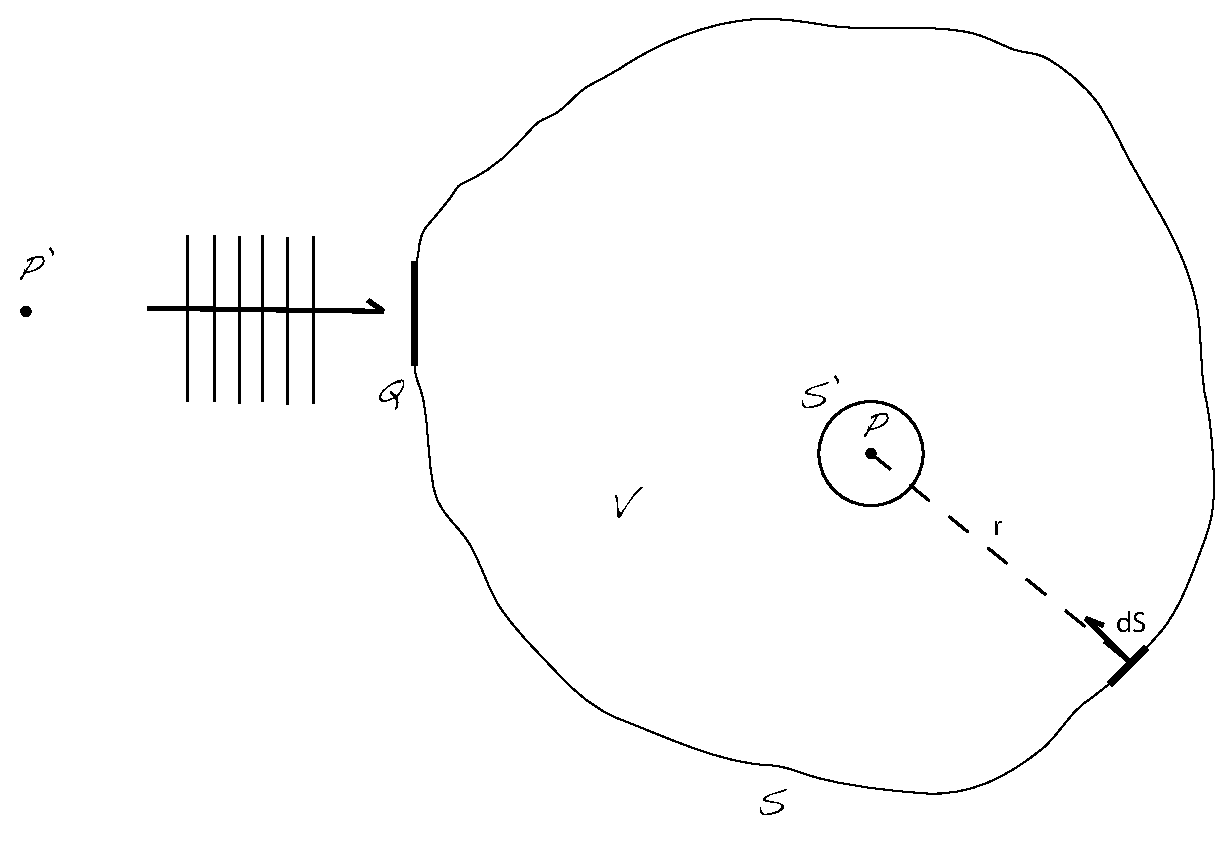
\psfig{file=helmholz-kirchhoff-surface.eps,width=0.7\textwidth}\hfil
	\centering
	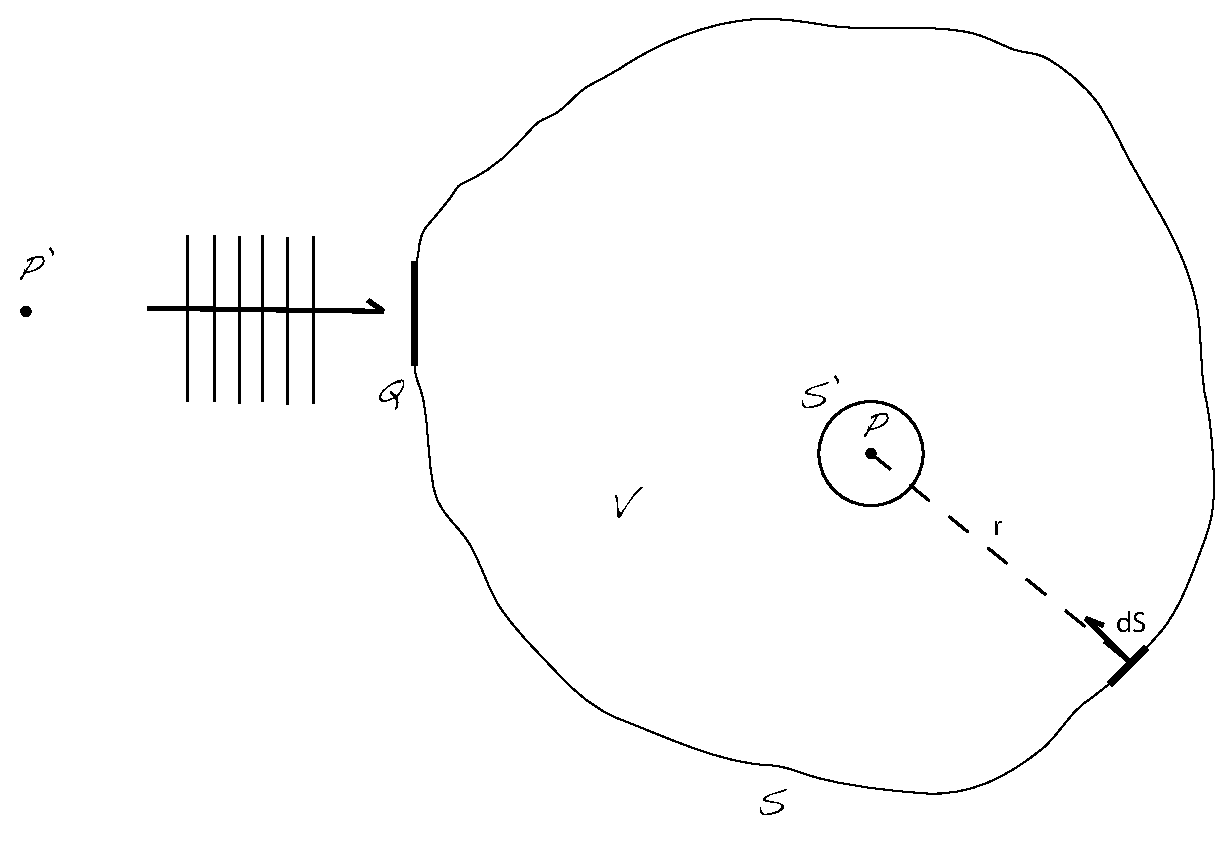
\includegraphics[width=0.7\textwidth]{helmholz-kirchhoff-surface.eps}
  \caption{Surface $\cal{S}$ for the Helmholtz-Kirchhoff integral. The surface
$\cal{S'}$ surrounds the observation point $\cal{P}$ and $\cal{V}$ is the 
volume bounded by $\cal{S}$ and $\cal{S'}$. The aperture $\cal{Q}$, the 
incoming wave to the left of it and the point $\cal{P'}$ are used later in the
text.}
  \label{fig:helmholz-kirchhoff-surface}
\end{figure}

The Helmholtz equation~\ref{eq:helmholtz} is an elliptic, linear, partial differential equation,
and thus permits us to express the value of $\psi_\cl{P}$ of $\psi$ at any point $\cl{P}$ inside
some closed surface $\cl{S}$ as an integral over $\cl{S}$ of some linear combination of $\psi$ 
and its normal derivative. 

Let us derive this expression by augmenting the actual wave $\psi$ in the interior of $\cl{S}$
with a second solution\footnote{Remember that in spherical polar coordinates we
write the gradient of a scalar as 
\[
\nabla f={\partial f\over\partial r}{\bf e}_r
     +{1\over r\sin\theta}{\partial f\over\partial\phi}{\bf e}_\phi
     +{1\over r}{\partial f\over\partial\theta}{\bf e}_\theta
\] 
and the divergence as 
\[
{\nabla\cdot A}={1\over r^2}{\partial\over\partial r}\left(r^2A_r\right)
+{1\over r\sin\theta}{\partial A_\phi\over\partial\phi}
+{1\over r\sin\theta}{\partial\over\partial\theta}(A_\theta\sin\theta)
\]} of the Helmholtz equation, namely
\[
\psi_0={e^{ikr}/r}.
\]
This is a spherical wave originating from the point $\cl{P}$, and $r$ is the distance from 
$\cl{P}$ to the point where $\psi_0$ is evaluated. Now apply Gauss' theorem 
\[
\int_\cl{V}\nabla\cdot{\bm F}dV=\int_\cl{S}{\bm F}\cdot d{\bm S}
\]
to the vector field $\psi\nabla\psi_0-\psi_0\nabla\psi$ and invoke Helmholtz equation to 
arrive at 
\[
\int_{\cl{S}+\cl{S}'}(\psi\nabla\psi_0-\psi_0\nabla\psi)\cdot d{\bm S}
           =-\int_\cl{V}(\psi\nabla^2\psi_0-\psi_0\nabla^2\psi)dV=0
\]
Where we have introduced a small sphere $\cl{S}'$ of radius $r'$ surrounding $\cl{P}$; $\cl{V}$
is the volume between the two surfaces $\cl{S}$ and $\cl{S}'$; and we have made the opposite 
choice of direction for the integration element $d{\bm S}$ -- it points into $\cl{V}$ instead
of outwardly as is usual, changing the sign of the second expression in the equation above. 

{\bf Exercise}

\begin{enumerate}
\item Confirm that the above expression is correct.
\newcounter{count}
\setcounter{count}{\value{enumi}} 
\end{enumerate}

Now let the radius $r'$ decrease to zero. We then find that 
\[
\psi\nabla\psi_0-\psi_0\nabla\psi\rightarrow {-\psi(0)/{r'}^2}+O({1/r'})
\]
and thus the integral over $\cl{S}'$ becomes $4\pi\psi(\cl{P})\equiv
4\pi\psi_\cl{P}$. 

{\bf Exercise}

\begin{enumerate}
\setcounter{enumi}{\value{count}}
\item Carry out the integration, and show that its value is $4\pi\psi_{\cl{P}}$.
\setcounter{count}{\value{enumi}} 
\end{enumerate}


Thus,
\be
\psi_\cl{P}={1\over 4\pi}\int_\cl{S}\left(\psi\nabla{e^{ikr}\over r}-{e^{ikr}\over r}\nabla\psi\right)\cdot d{\bm S}.
\label{eq:helmholtz-kirchoff}
\ee

This equation is the {\it Helmholtz-Kirchhoff formula} is the expression relating $\psi$ at 
$\cl{P}$ to a linear combination of its value and normal derivative on a surrounding surface.
If $\cl{P}$ is many wavelengths away from the boundary $\cl{S}$, then the integral is only 
influenced by the waves $\psi$ as they enter through $\cl{S}$, and not when they are
leaving.

\subsection{Diffraction by an aperture}

Next let us suppose that some aperture $\cl{Q}$ of size much greater than a wavelength but
much smaller than the distance to $\cl{P}$ is illuminated by a distant wave source. Let 
$\cl{S}$ pass through $\cl{Q}$, and denote by $\psi'$ the wave incident on $\cl{Q}$. Assume
that the diffracting aperture has a local and linear effect on $\psi'$: that the wave 
transmitted through the aperture is given by 
\[
\psi_\cl{Q}=t\psi',
\]
where $t$ is a complex transmission function that varies over the aperture. In practice, $t$
is usually zero or unity. However, $t$ can also represent a variable phase factor when, for
example, the aperture comprises a medium of variable thickness and of different refractive
index from that of the homogeneous medium outside the aperture.

Let us now use the Helmholtz-Kirchhoff formula~\ref{eq:helmholtz-kirchoff} to compute the field
at $\cl{P}$ due the the wave $\psi_\cl{Q}=t\psi'$ transmitted through the aperture. The
surface $\cl{S}$ comprises the aperture $\cl{Q}$, a sphere of radius $R\gg r$ centered on 
$\cl{P}$, and the linear extension of the aperture to meet the sphere; and assume that the only
incoming waves are those which pass through the aperture. 

On the aperture, as $kr\gg 1$, we can write $\nabla({e^{ikr}/r})\simeq -{ik{\bm n}e^{ikr}/r}$ 
where ${\bm n}$ is a unit vector pointing towards $\cl{P}$. Similarly we write 
$\nabla\psi\simeq ikt{\bm n'}\psi'$, where ${\bm n'}$ is a unit vector along the direction
of propagation of the incident wave (and where our assumption that anything in the aperture
varies on scales long compared to $\lambda={1/k}$ permits us to ignore the gradient of $t$).
Inserting these gradients into equation~\ref{eq:helmholtz-kirchoff} one obtains
\be
\psi_\cl{P}=-{ik\over 2\pi}\int_\cl{Q}d{\bm S}\cdot\left({{\bm n}+{\bm n'}\over 2}\right){e^{ikr}\over r}t\psi'
\label{eq:small-aperture}
\ee
This equation can be used to compute the wave from a small aperture at any point $\cl{P}$ in 
the far field. It has the form of an integral transform for the incident field variable $\psi'$,
where the integral is over the area of the aperture. The kernel of the transform is the 
product of several factors: the factor ${1/r}$ ensures that the flux or energy (proportional
to $\psi^2$) falls off as the inverse square of the distance to the aperture. The phase 
factor $-ie^{ikr}$ advances the phase of the wave by an amount equal to the optical path 
length between the element of the aperture and $\cl{P}$, minus ${\pi/2}$. The amplitude and
phase of the incoming wave $\psi'$ can also be changed by the transmission function $t$.
Finally there is the {\it obliquity factor} ${d\hat{\bm S}\cdot({\bm n}+{\bm n'})/2}$, where 
$d\hat{\bm S}$ is the unit vector normal to the aperture. 

\subsection{Spreading of the Wavefront}

Equation~\ref{eq:small-aperture} gives a general description for computing the diffraction 
pattern from an illuminated aperture. It is commonly used in two different limits, called
{\it Fraunhofer} and {\it Fresnel}.

Suppose that the aperture has a linear size $a$ and is roughly centered on the geometric ray
from the the source point $\cl{P}'$ to the field point $\cl{P}$. Consider the variations of 
the phase $\phi$ of the contributions to $\psi_\cl{P}$ that come from various places in the
aperture. Using trigonometry we can estimate that locations on opposite sides of the aperture
produce phases at $\cl{P}$ that differ by $\Delta\phi=k(r_2-r_1)\sim {ka^2/2r}$, where $r_1$ and
$r_2$ are the distances from the two edges of the aperture to the point $\cl{P}$. 

{\bf Exercise}

\begin{enumerate}
\setcounter{enumi}{\value{count}}
\item Why can we write $(r_2-r_1)\sim a^2/2r$? Draw a figure to show
  the geometry of the problem.
\setcounter{count}{\value{enumi}} 
\end{enumerate}

There are
two limiting regimes depending on whether the aperture is large or small compared with the 
{\it Fresnel length}
\[
r_{F}\equiv\left({2\pi r\over k}\right)^{1/2}=(\lambda r)^{1/2}
\]
When $a\ll r_{F}$, the phase variation $\Delta\sim {a^2/r_{F}^2}$ is $\ll \pi$ and can be 
ignored; the contributions from different parts of the aperture are essentially in phase with
each other -- this is the {\it Fraunhofer} regime. When $a\gg r_{F}$, $\Delta\phi\gg \pi$ and the 
phase variation is very important in determining the observed intensity 
$\labs\psi_\cl{P}\rabs^2$ -- this is the {\it Fresnel} regime.

Consider a planar wave propagating perpendicular to an aperture of size $a$. 
Wave optics insists that the transverse localization of the wave into a region of size
$\Delta x\sim a$ must produce a spread in its transverse wave vector, $\Delta k_x\sim{1/a}$
(a momentum of uncertainty\footnote{In this way
we can achieve a quick and dirty ``derivation'' of the Rayleigh criterion using photons with
momentum $p$ impinging on a lens of diameter $a$ which gives that the resolution 
($\theta=\Delta p_x/p$) may be found as 
\[
\theta={\Delta p_x/p}={{h/a}\over{h/\lambda}}={\lambda/a}.
\]} $\Delta p_x=\hbar\Delta k_x\sim{\hbar/a}$.)
This uncertain transverse vector produces, after propagating a distance $r$,
a corresponding uncertainty $({\Delta k_x/k})r\approx {r_{F}^2/a}$ in the beam's transverse 
size; and this uncertainty superposes incoherently on the aperture-induced size $a$ to 
produce a net transverse beam size 
\bua
\Delta x&\sim&\sqrt{a^2+({r_{F}^2/a})^2} \\
        &\sim&a\qquad{\rm if}\quad r\ll {a^2/\lambda}\quad{\rm Fresnel~regime} \\
        &\sim&\left({\lambda\over a}\right)r\qquad{\rm if}\quad r\gg {a^2/\lambda}\quad{\rm Fraunhofer~regime}.
\eua
In the nearby Fresnel regime the aperture creates a beam whose edges will have the same shape and
size as the aperture itself, and will be reasonably sharp but with some oscillatory blurring
associated with wave-packet spreading. By contrast in the more distant Fraunhofer regime wave
front spreading will cause the transverse size of the entire wave to grow linearly with the 
distance, and the intensity pattern will typically not resemble the aperture at all.

\subsection{Fraunhofer Diffraction}

\begin{figure}[th!]
%  \hfil\psfig{file=path-length.eps,width=0.7\textwidth}\hfil
	\centering
	\includegraphics[width=0.7\textwidth]{path-length.eps}
  \caption{Geometry for computing the path length between a point $\cal{Q}$ in 
the aperture and the observation point $\cal{P}$. The transverse vector 
$\bf{x}$ is used to identify $\cal{Q}$ in the Fraunhofer analysis and in a
later lecture $\bf{x'}$ is used for Fresnel analysis.}
  \label{fig:path-length}
\end{figure}

Consider now the Fraunehofer regime and specialize to the case of an incident plane wave with
 wave vector ${\bm k}$ orthogonal to the aperture plane. Regard the line along ${\rm k}$ through
the center of the aperture $\cl{Q}$ as the ``optic axis''; identify points in the aperture by
their two-dimensional vectorial separation ${\bm x}$ from that axis; identify $\cl{P}$ by 
its distance $r$  (note change in definition of $r$) 
from the aperture center and its 2-dimensional transverse separation 
$r{\bm\theta}$ from the optic axis. Now, restrict attention to small angle diffraction
$\labs{\bm\theta}\rabs\ll 1$. The geometric path length between $\cl{P}$ and a point ${\bm x}$ on 
$\cl{Q}$ can be expanded as
\[
{\rm Path~length}=(r^2-2r{\bm x}\cdot{\bm\theta}+x^2)^{1/2}
       \simeq r-{\bm x}\cdot{\bm\theta}+{x^2\over 2r}+\ldots
\]
The first term in this expression, $r$, just contributes an ${\bm x}$-independent phase
$e^{ikr}$ to $\psi_\cl{P}$. The third term, ${x^2/2r}$, contributes a phase variation that is
$\ll 1$ here in the Fraunenhofer region (but will be important in the Fresnel region). Therefore, 
in the Fraunhofer region, we can retain just the second term $-{\bm x}\cdot{\bm\theta}$ and
write equation~\ref{eq:small-aperture} 
\[
\psi_\cl{P}({\bm\theta})\propto\int e^{-ik{\bm x}\cdot{\bm\theta}}t({\bm x})d^2x
     \equiv\bar{t}({\bm\theta})
\]
Where $d^2x$ is the surface area element in the aperture plane and we have dropped a constant
phase factor and constant multiplicative factors. Thus, $\psi_\cl{P}({\bm\theta})$ in the 
Fraunhofer regime is given by the two dimensional Fourier transform denoted by 
$\bar{t}({\bm\theta})$, of the transmission function $t({\bm x})$, with ${\bm x}$ made 
dimensionless in the transform by multiplying with $k={2\pi/\lambda}$. 

\subsection{Diffraction of a single slit}

Consider now a single transparent stripe, a slit, of width $a$ centered on $x=0$, and 
measure the scalar angle $\theta$ from the direction of the incident radiation. This slit
has the transmission function 
\bua
t_1(x)&=&1\quad\labs x\rabs<{a/2}, \\
      &=&0\quad\labs x\rabs>{a/2}.
\eua
Its diffraction pattern is 
\bua
\psi_\cl{P}({\bm\theta})&\propto&\bar{t}_1 \\
                        &\propto&\int_{-{a/2}}^{a/2}e^{ikx\theta}dx \\
                        &\propto&{\rm sinc}\left({ka\theta\over 2}\right),
\eua
where ${\rm sinc}(x)\equiv{\sin(x)/x}$. 

{\bf Exercise}

\begin{enumerate}
\setcounter{enumi}{\value{count}}
\item Carry out the intergration $\int_{-{a/2}}^{a/2}e^{ikx\theta}dx$  above, and show that the result is correct. 
\item The intensity of radiation is proportional to the square of
  $\psi$. Plot, for example with {\sc IDL}, the intensity pattern from
  the diffraction of a single slit in the Frauhofer regime.
\setcounter{count}{\value{enumi}}
\end{enumerate}

\subsection{Babinet's principle}

In the previous section we have shown how to compute the Fraunhofer diffraction pattern formed
by a narrow slit. We might also be interested in the pattern produced by the complementary
aperture, {\it i.e.} a needle of width and length the same as the slit. We can derive the 
needles pattern by observing that the sum of the waves from the two apertures should equal the
wave from a completely unaltered incident wave front. That is to say if we exclude the
direction of the incident wave, the field amplitude diffracted by the two apertures are the
negative of each other, and hence the intensities $\labs\psi\rabs^2$ are the same. 
Therefore the Fraunhofer diffraction patterns from the needle and the slit --- and indeed from
any complementary apertures --- are identical, except in the direction of the incident 
wave.

\subsection{Diffraction by a circular aperture}

Let us now compute how well a telescope can distinguish neighboring stars. We cannot expect to
resolve them (or any two objects) that are closer together in the sky than the angular width
of the diffraction pattern formed by the telescope's aperture. Of course, optical imperfections
and pointing errors in a real telescope may degrade the image quality even further, but this
is the best that can be done, limited only by the uncertainty principle.

\begin{figure}[th!]
%  \hfil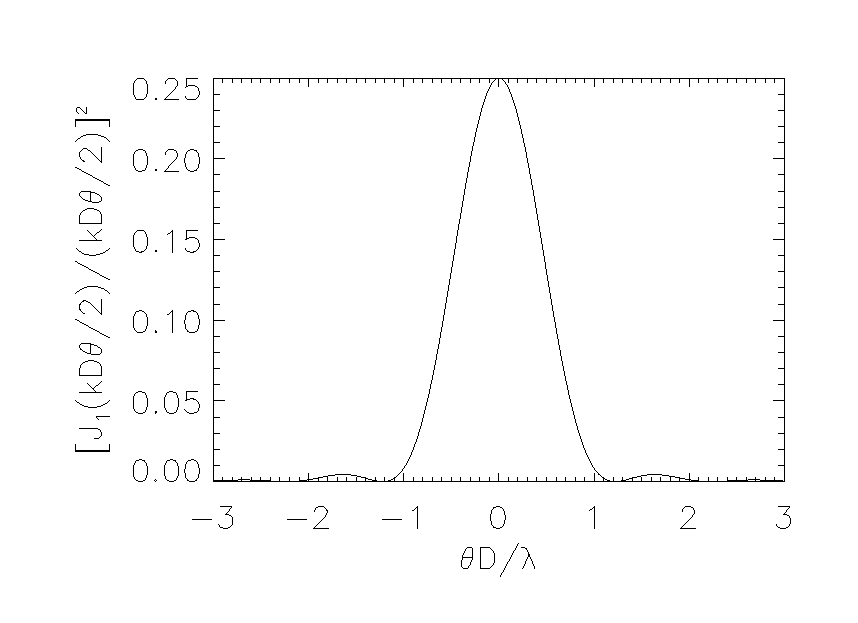
\psfig{file=jinc2.eps,width=0.7\textwidth}\hfil
	\centering
	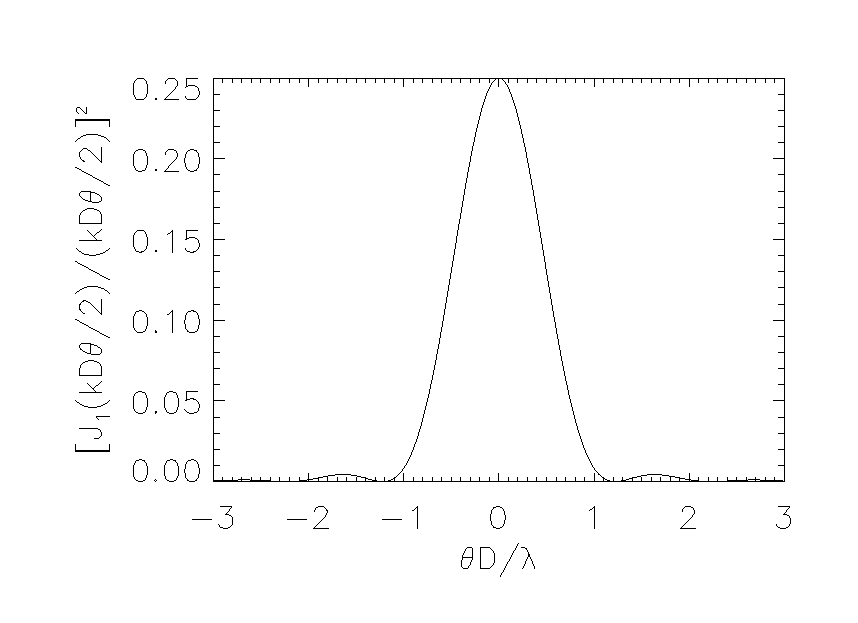
\includegraphics[width=0.7\textwidth]{jinc2.eps}
  \caption{Airy diffraction pattern for a circular aperture. Note the first zero
of the function at $\theta D/\lambda=1.22$.}
  \label{fig:jinc2}
\end{figure}

The calculation is straightforward using equation~\ref{eq:small-aperture} and assuming a circular
aperture telescope with diameter $D$:
\bua
\psi(\theta)&\propto&\int_{\pi D}e^{-ik{\bm x}\cdot{\bm\theta}}d^2x \\
            &\propto&{\rm jinc}\left({kD\theta\over 2}\right)
\eua
where ${\rm jinc}(x)\equiv {J_1(x)/x}$ with $J_1$ the Bessel function of order one. The
flux from an star observed at angle $\theta$ is therefore $\propto{\rm jinc}^2({kD\theta/2})$.
This intensity pattern is known as the {\it Airy pattern}. There is a central ``Airy disk'' 
surrounded by a circle where the flux vanishes, and then further surrounded by a series of 
concentric rings whose flux vanishes with radius. Only 16\% of the tatal light falls outside
the the central Airy disk. The angular radius $\theta_A$ of the Airy disk, {\it i.e.} the 
radius of the dark circle surrounding it, is determined by the first zero of 
$J_1({kD\theta/2})$ which is found to be $\theta_A={1.22\lambda/D}$. 

{\bf Exercise}

\begin{enumerate}
\setcounter{enumi}{\value{count}}
\item Write a {\tt IDL} routine that plots a cut through the Airy disk such as figure~\ref{fig:jinc2}
and, in addition, plots an image of the Airy disk.
\setcounter{count}{\value{enumi}}
\end{enumerate}

%\end{document}
